\justifying
\NSFCBodyText

\subsubsection{研究背景与意义}
\textbf{项目名称：面向长程多步骤智能体的自适应上下文压缩、动态卸载与按需证据恢复研究（ACORE）。}本项目围绕 CCF—快手大模型探索者基金课题“Agent 上下文工程：面向多步骤任务的上下文压缩与卸载技术研究”，研究有限上下文下的长程行动可靠性。拟以现有大语言模型为执行主体，建立能够保留任务状态、按需回取有效证据并控制总调用开销的上下文管理方法。

多步骤智能体需要持续读取工具结果、维护未完成目标，并根据环境反馈修订行动。ReAct 将推理与行动交替组织，使模型能够利用外部观察推进任务\cite{react}；Toolformer 和 ToolLLM 进一步展示了学习工具选择与接口使用的可行性\cite{toolformer,toolbench}。这些能力使智能体可承担信息检索、代码修改和跨工具协作，也使任务历史不断累积。一次检索可能返回多篇文档，一次测试可能产生长日志；只有少量信息与当前动作相关，而早先出现的约束仍可能决定后续操作是否正确。

例如，一个拟构建的跨工具测试任务要求智能体核对订单状态、读取适用政策并更新记录。早期观察包含对象标识、状态版本和禁止重复处理的约束，中间插入大量无关日志，后续政策又发生更新。若压缩只留下“已核对订单”这一概括，系统可能忘记适用对象或再次执行已完成动作；若恢复时取回内容相似的旧政策，即使字节完整，也可能作出不再满足当前条件的操作。这一例子是研究情境示意，不代表已有企业数据或前期实验。它揭示了需要同时回答的三个问题：压缩后哪些状态仍应可见，卸载证据如何恢复为当前可用的信息，以及这一过程是否值得付出额外成本。

上下文管理的价值因而包含两个相互制约的方面。一方面，减少工具噪声和重复历史有望降低资源消耗，缓解关键信息被淹没的问题；另一方面，压缩可能损失对象关系、时间条件和行动前提，使错误在长程执行中累积。Lost in the Middle 发现关键信息位置能够影响长上下文任务表现\cite{lostmiddle}，说明名义窗口长度不能代替有效利用能力。但不同模型与任务的敏感性并不相同，不能据此推断所有长历史都应被强压缩。需要将任务状态、证据更新和资源约束放在同一实验条件下分析，寻找能够保持可靠行动的压缩范围。

本研究的科学价值在于解释\textbf{压缩后保留的动作依赖、回取证据的当前有效性与任务失败风险之间的关系}，并用受控干预检验这一关系。技术价值在于形成可接入现有文本与工具调用智能体的上下文管理原型，给出何时应压缩、何时值得恢复、何时应保留完整证据的可复核依据。公开环境中的可重复结论构成核心交付，企业业务验证在数据和接口授权落实后开展。

\subsubsection{国内外研究现状及发展动态分析}
\textbf{提示压缩为资源节省提供了方法基础，但跨步信息价值需要另外判断。}Selective Context 依据自信息量过滤内容\cite{selectivecontext}；LLMLingua 通过预算控制与逐词筛选压缩提示\cite{llmlingua}，LongLLMLingua 进一步考虑查询相关性、信息密度和位置偏差\cite{longllmlingua}。LLMLingua-2 将保留决策蒸馏为较小模型的词级分类任务，以降低压缩开销并改善跨任务适用性\cite{llmlingua2}。在检索增强场景中，RECOMP 联合使用文本压缩与选择性增强，使送入主模型的内容更紧凑\cite{recomp}。这些方法适合用作本项目的轻量基线，但静态问句中的信息显著性未必等价于未来动作所需的信息价值；将它们直接用于长程轨迹时，需要检验被删除的内容是否参与尚未完成的依赖关系。

\textbf{轨迹压缩已经开始显式利用任务状态与失败反馈。}ACON 针对观察和历史记录联合压缩，利用失败案例改进自然语言压缩指南，并研究小模型压缩器蒸馏\cite{acon}。它已关注保留关键环境信息，不能将“从文本压缩走向任务状态保持”笼统作为本项目独有贡献。AgentFold 通过细粒度凝练与跨步骤合并形成多尺度状态摘要，将主动上下文整理与任务行动结合\cite{agentfold}。两者分别提供失败驱动和轨迹折叠的直接比较对象。值得进一步追问的是，显式保留未完成动作的证据依赖，是否在相同摘要长度与候选证据条件下仍能降低后续违例；如果作用只是增加了上下文长度或查询次数，就不能将其归结为新的保真机制。

\textbf{长期记忆与按需原文回取已有多种实现。}MemoryBank 通过更新和遗忘机制组织历史信息\cite{memorybank}；Generative Agents 将经历记录、反思和动态检索结合\cite{generativeagents}。MemGPT 借鉴分层存储，在工作上下文与外部记忆之间移动信息\cite{memgpt}。ReadAgent 生成关联原文位置的摘要记忆，再按任务需要回读原始段落\cite{readagent}，已经覆盖“保留概要、按需恢复细节”的基本思路。A-MEM 通过笔记链接和记忆演化组织信息\cite{amem}，Mem0 研究结构化抽取、整合和检索\cite{mem0}。因此，可寻址存储、摘要回读或记忆图结构本身均不足以支撑本申请的创新论断。

检索增强生成和稠密检索为外部证据访问提供基础\cite{rag,dpr}，Self-RAG 将检索和反思与任务需求结合\cite{selfrag}。然而，对会修改环境的任务，语义相关的片段仍可能描述旧状态。近期 MemStrata 已直接讨论检索记忆的时间有效性\cite{memstrata}；PLACEMEM 包含版本化记忆、来源信息和失效传播，并讨论算力与记忆组织的关系\cite{placemem}；Agent Zero Memory 进一步研究来源可追溯的长期记忆\cite{agentzero}。最新的 Invalidation Contracts 已讨论带版本信息的记忆失效与使用规则\cite{invalidation}，From Faulty Memories to Corrected Actions 把记忆与动作关系用于纠错及选择性回放\cite{rollbackrepair}。这些工作要求本项目将问题收窄到\textbf{压缩造成的动作依赖缺失如何与恢复证据的有效性共同影响真实操作}，而不能把版本管理或来源追溯单独包装成新机制。

\textbf{统一记忆调度已进入学习型决策阶段，仍需检验总开销下的收益边界。}Reflexion 表明自然语言反馈能够影响后续尝试\cite{reflexion}；Memory-R1 利用结果反馈学习记忆管理和选用\cite{memoryr1}；AgeMem 将长期与短期记忆操作纳入同一策略，研究渐进训练与步骤级奖励\cite{agemem}。ContextBudget 已明确研究预算约束下的长程搜索上下文管理\cite{contextbudget}。本项目不以“统一压缩、卸载和恢复”这一结构名称主张原创性，而关注在固定执行模型后，动作依赖和证据有效性带来的可靠性改善能否覆盖压缩器、检索、验证及重试成本。What Does Context Compression Cost an Agent 已指出压缩后的重新取证可能增加交互代价\cite{compressioncost}。因此，全开销统计属于必要比较原则，拟研究的增量是元数据不完全可见时，有限预算应怎样分配给依赖保留与主动重查。

\textbf{评价对象正从长文理解扩展到记忆与交互终态。}LongBench 为双语长上下文理解提供多任务测试\cite{longbench}，RULER 通过多跳追踪和信息聚合检验超出简单查找的能力\cite{ruler}。LongMemEval 覆盖信息抽取、多会话推理、时间推理、知识更新和拒答\cite{longmemeval}，LoCoMo 考察长期会话记忆\cite{locomo}。这些测试有助于定位压缩与恢复错误，但问答正确不能直接证明工具操作正确。AppWorld 使用可控应用环境及数据库终态测试判断任务是否完成\cite{appworld}，WebArena 提供可复现的网页交互环境\cite{webarena}。AgentBench 支持跨环境能力诊断\cite{agentbench}，SWE-bench 和 GAIA 分别提供代码修改及多工具任务的扩展评测参照\cite{swebench,gaia}。\(\tau\)-bench 对规则遵从与多次运行可靠性的评价\cite{taubench}进一步说明，任务完成率、重复运行稳定性和过程指标需要分别报告。

\subsubsection{现有研究的不足}
现有工作留下的研究空间，主要体现在\textbf{机制证据的连接}。压缩研究常报告长度和终态表现，记忆研究常报告检索或问答表现，版本管理研究则强调更新和失效处理。对连续操作环境，需要进一步区分：压缩是否删去了动作前提，检索是否遗漏正确片段，候选证据是否已经过期，以及执行模型在获得有效证据后是否仍选择错误动作。只有将这些环节分离，才可能判断改进来自何处、何时失效。本项目把这一点视为在本次已核验文献集合上的研究切入判断，不宣称相关问题从未被研究。

第二，关于可恢复性的论证容易混合不同层次。外部存储保留原文，只能提供重新读取的可能；内容哈希一致，只能证明读回字节与存入内容一致。动作真正需要的是对象、适用条件和版本均匹配的证据。当执行环境变化、索引滞后或元数据缺失时，找到旧证据反而可能使模型更加确信错误判断。因此，研究需要让恢复机制接受环境终态的检验，并将“检索到了”“版本有效”“动作正确”分别统计。

第三，成本比较容易遗漏控制过程。更多检索和更强验证可能提高任务成功率，却增加总体调用开销；反复压缩还可能将一次长输入的成本转化为多次短调用。不同基础模型、缓存策略和重试次数也会混淆比较。应固定执行模型与任务集合，先做相同候选证据和回取开销的机制比较，再做完整系统比较，并预先规定超时、拒答与资源耗尽的计分方式。

\subsubsection{关键科学问题与研究切入点}
本项目的中心科学问题是：\textbf{在有限上下文与总调用预算下，压缩后动作依赖的保留和恢复证据的有效性怎样共同影响长程智能体的任务失败风险，这种改善在什么条件下仍具有净收益？}其中，拟重点检验元数据只部分可见而当前状态仍可查询时，有限预算在依赖保留与主动取证之间应如何配置。围绕这一问题提出三个子问题：未完成动作所依赖的约束能否比文本显著性更准确地识别应保留信息？恢复时结合动作前提与当前环境版本，能否降低过期证据驱动的操作失败？额外压缩、检索和校验开销在何种任务长度、依赖跨度及更新频率下能够被抵消？
% NSFC-ILLUSTRATED BEGIN F01
如图~\ref{fig:background} 所示，长程任务的状态遗漏、证据失效与控制开销构成三项研究的切入点。
\begin{figure}[htbp]
\centering
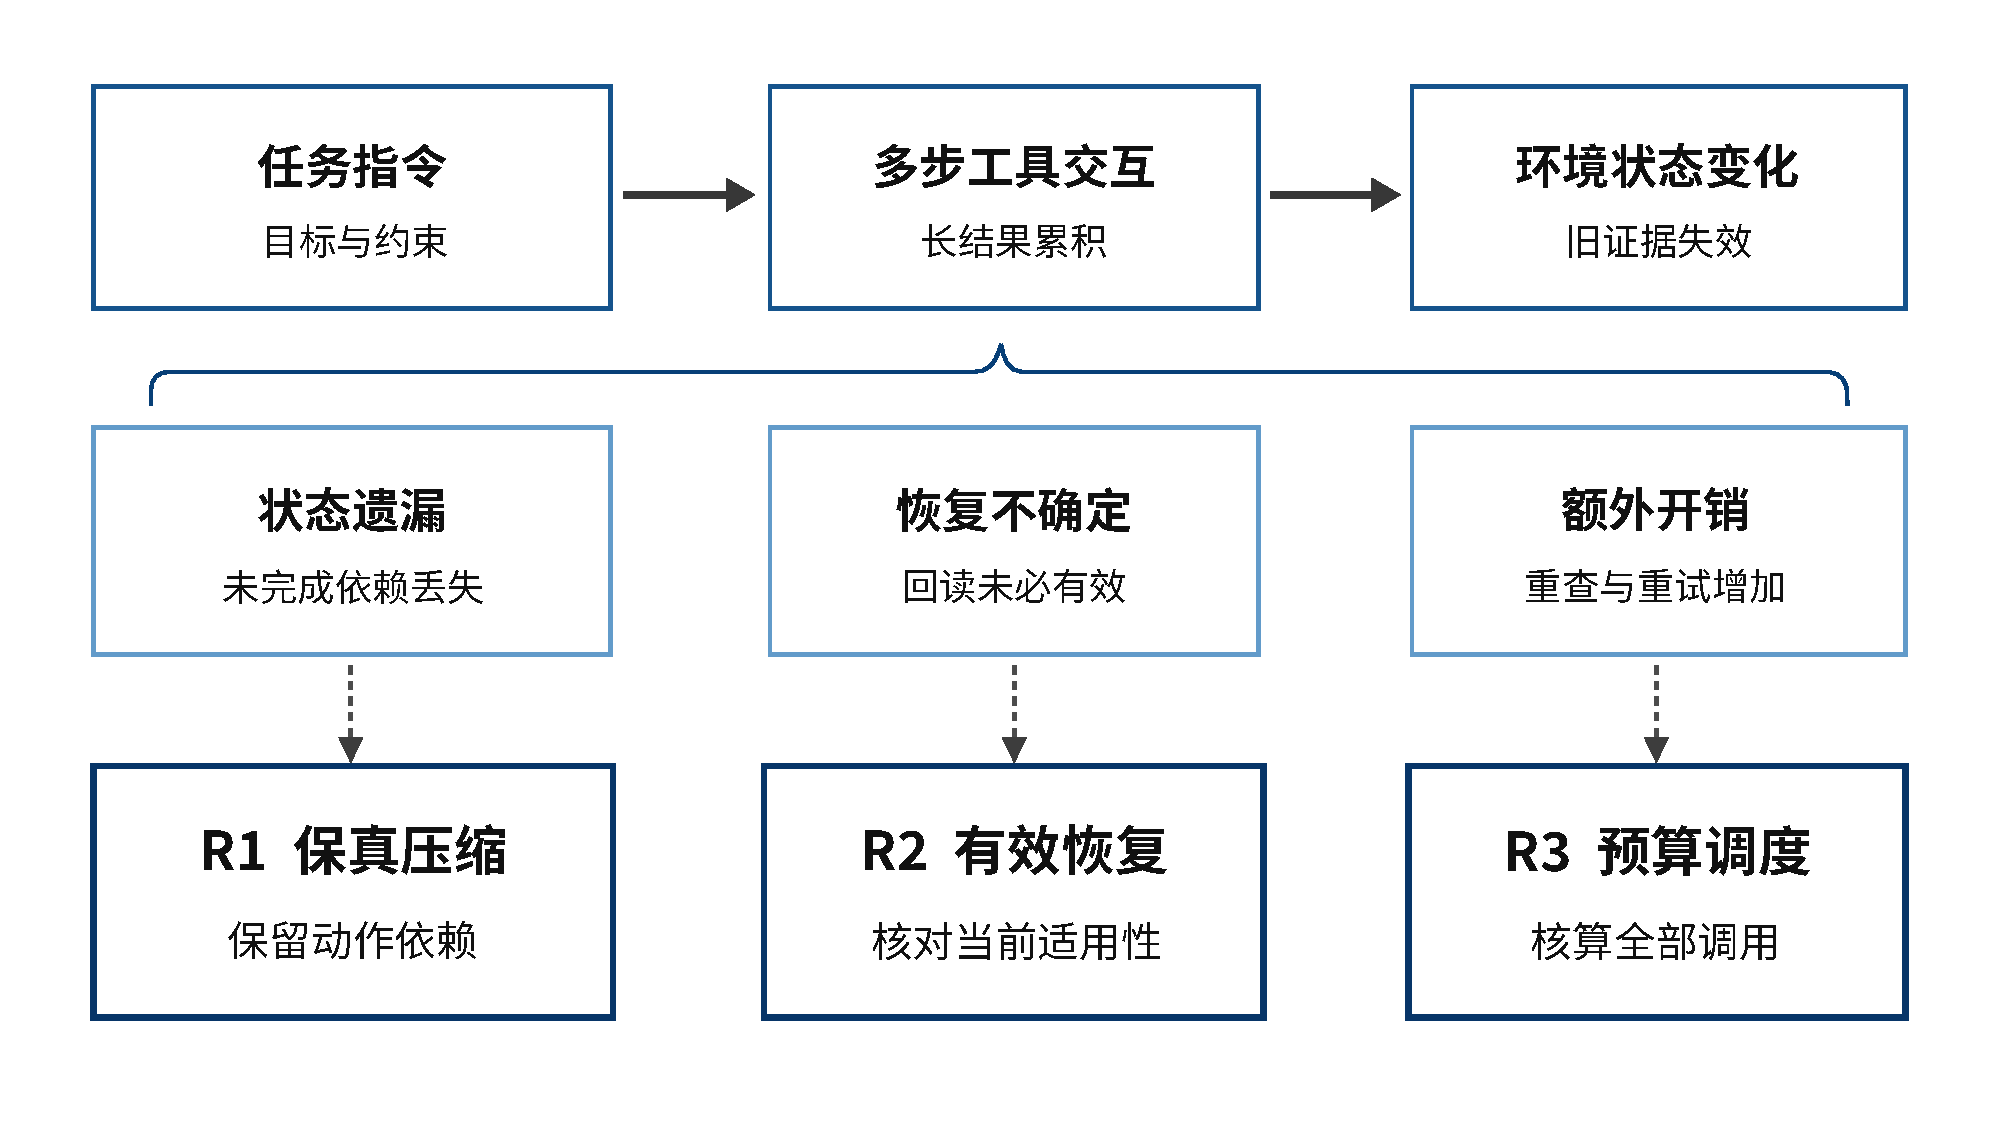
\includegraphics[width=0.98\linewidth]{figures/F01-background.pdf}
\caption{长程任务的状态遗漏、证据失效与控制开销构成三项研究的切入点}
\label{fig:background}
\end{figure}
% NSFC-ILLUSTRATED END F01


据此提出待检验假说：在相同执行模型、窗口预算与原文存储条件下，保留未完成动作的证据依赖，并在恢复时核对动作前提与证据版本，将在跨阶段依赖较强且环境经常更新的任务中降低终态失败风险；这种改善在静态、短程任务中可能减弱，额外控制开销也可能使净收益消失。通过“依赖保留有无”与“有效性校验有无”的交叉对照，检验组合效果是否超出简单模块叠加。如果在匹配候选证据、上下文长度和恢复开销后差异消失，或经调优的简单规则达到同等效果，将收缩相应机制主张。

在版本号、依赖关系或有效期不完整的实际接口中，保留更多关系会挤占上下文，减少关系又可能增加重查次数。本项目进一步将压缩强度、依赖可见程度和元数据错漏作为分层条件，检验有限Token在保留与主动取证之间的配置规律。所有方法获得相同真实元数据；完整环境状态只供诊断标注，不单独向本方法开放。当前状态既不可观察又不可重查时，研究不主张保证动作正确。

研究由三项相互衔接的内容组成：任务状态感知的保真压缩、动作依赖引导的证据卸载与有效恢复、计及全开销的自适应调度与可靠性验证。前一项为后一项提供状态及不确定性依据，恢复结果又反馈给调度器更新保留与回取决策。预期贡献是形成这一关系的实验依据、可复用方法与适用边界，避免将原型开发或尚未取得的业务提升当作已验证成果。
